% 2007 年福建卷理科第 18 题：正三棱柱 ABC-A1B1C1（底面正三角形、侧棱垂直底面，
%   所有棱长均为 2），D 为 CC1 的中点；图中画出 AB1、A1B、A1D、BD 等辅助线。
% 来源 PDF：gaokaomath-src/普通高考/2007/2007福建理.pdf
% SHA-256：e9ade36d1b1e3154a7e37226957037a45635faeedcfb823df216fceabcc5a1dc
% 原页：2007福建理.pdf 第 1 页（A3 三栏）第 3 栏，书页码 367。
% 重绘依据：按原页横放的三棱柱（左三角面 ABC、右三角面 A1B1C1）与虚线重绘；
%   C 为被遮挡的后顶点，A-C、B-C、C-C1 画虚线，D 取 CC1 中点。
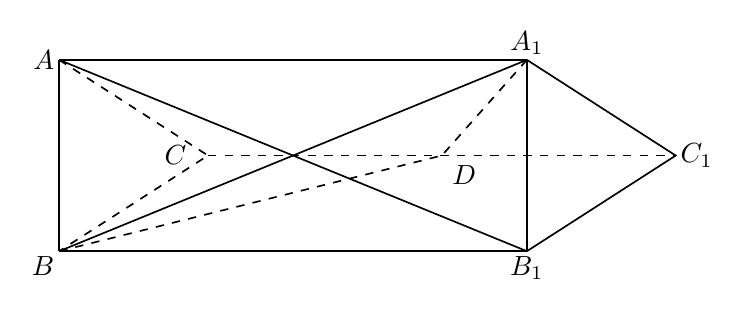
\begin{tikzpicture}[scale=0.9, semithick,
  every node/.style={inner sep=1.5pt}]

  \coordinate (A)  at (0.0,2.7);
  \coordinate (B)  at (0.0,0.0);
  \coordinate (C)  at (2.1,1.35);
  \coordinate (A1) at (6.6,2.7);
  \coordinate (B1) at (6.6,0.0);
  \coordinate (C1) at (8.7,1.35);
  \coordinate (D)  at (5.4,1.35);

  % 左三角面
  \draw (A) -- (B);
  \draw[dashed] (A) -- (C) -- (B);
  % 侧棱
  \draw (A) -- (A1);
  \draw (B) -- (B1);
  \draw[dashed] (C) -- (C1);
  % 右三角面
  \draw (A1) -- (B1);
  \draw (A1) -- (C1) -- (B1);
  % 题设辅助线
  \draw (A) -- (B1);
  \draw (A1) -- (B);
  \draw[dashed] (A1) -- (D);
  \draw[dashed] (B) -- (D);

  \node[left] at (A) {$A$};
  \node[below left] at (B) {$B$};
  \node[left=6pt] at (C) {$C$};
  \node[above] at (A1) {$A_1$};
  \node[below] at (B1) {$B_1$};
  \node[right] at (C1) {$C_1$};
  \node[below right=2pt] at (D) {$D$};
\end{tikzpicture}
